\subsection{Comparison with EMV2}
\label{subsec:comparison_with_EMV2}

The AADL language has previously been extended to provide some fault modeling and analysis capabilities using its Error Model Annex, Version 2 (EMV2)~\cite{EMV2}.  EMV2 focuses on injection and propagation of discrete faults for generation of fault trees, rather than on analysis of system behavior in the presence of faults. In the EMV2 approach, all faults must be explicitly propagated through each component (by applying fault types on each of the output ports) in order for a component to have an impact on the rest of the system. When using this type of fault analysis, the safety analyst must understand the system  behavior and component functions well enough to specify how a failure will propogate through the system, what the destination components reaction to said failure will be, and correctly implement these propagations. In EMV2, every possible component failure must be specified in this way. As a contrast, the Safety Annex provides two ways in which to specify these faults. The explicit propagation capability in the Safety Annex is meant to capture hardware faults and faults that occur due to colocated components. In every other instance, implicit propagation is used through the behavior model. In related work, comparisons with other related toolsets is explored in more depth. 














\iffalse

The AADL language has previously been extended to provide some fault modeling and analysis capabilities using its Error Model Annex, Version 2 (EMV2)~\cite{EMV2}.  EMV2 focuses on injection and propagation of discrete faults for generation of fault trees, rather than on analysis of system behavior in the presence of faults. 
To illustrate some of the key differences between our approach and the EMV2 approach, Figure~\ref{fig:comparison_with_EMV2} shows a simplified example based on an aircraft Wheel Brake System (WBS). The WBS model is described in greater detail in ~\cite{Stewart17:IMBSA} and in Section \ref{sec:case_study}. The code fragments in the figure extracted from EMV2, AGREE, and the Safety Annex do not represent the complete code.

\begin{figure}[t]
	\vspace{-0.19in}
	\centering
	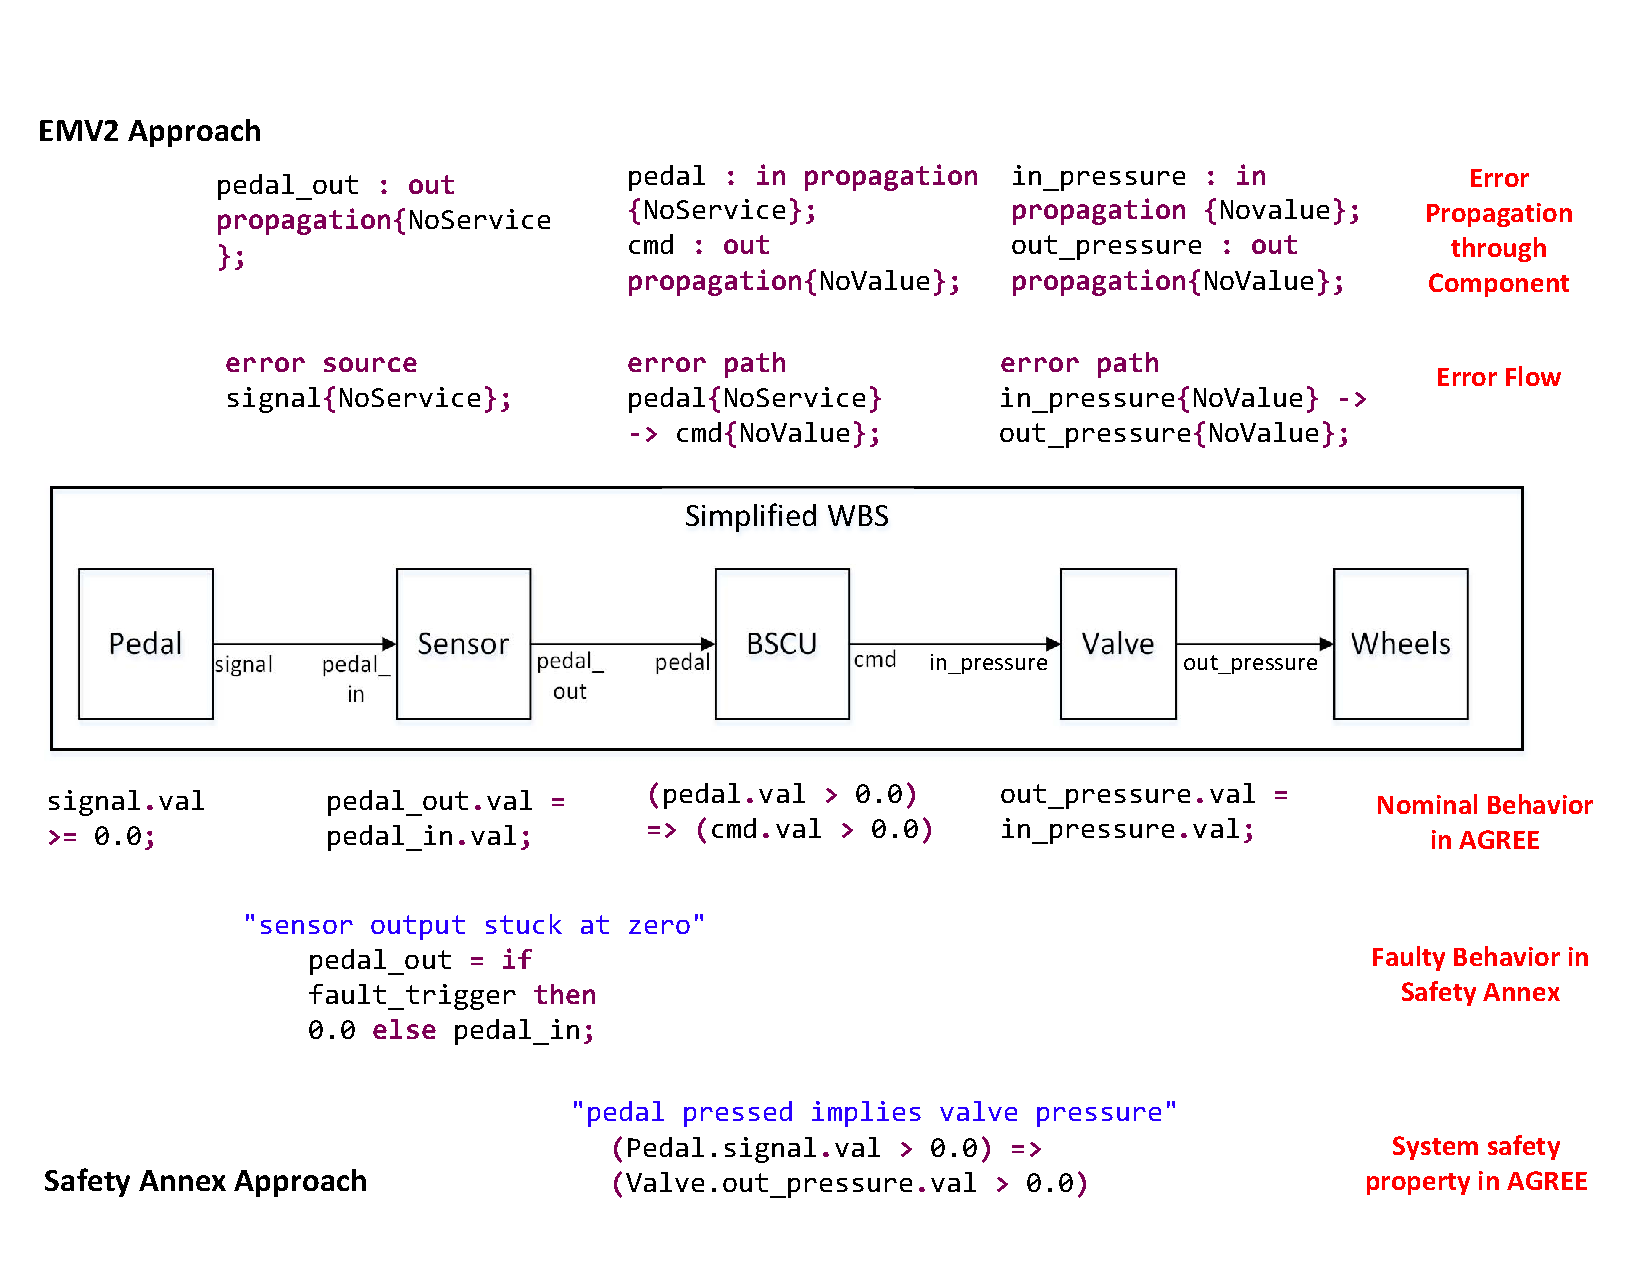
\includegraphics[trim=0 9 0 5,clip,width=\textwidth]{images/Comparison_with_EMV2.pdf}
	%\vspace{0.4in}
	\caption{Differences between Safety Annex and EMV2}
	\label{fig:comparison_with_EMV2}
\end{figure} 

In our simplified WBS system, the physical signal from the Pedal component in detected by the Sensor, and the pedal position value is passed to the Braking System Control Unit (BSCU) components.  The BSCU generates a pressure command to the Valve component which applies hydraulic brake pressure to the Wheels. In this example, we use the general term ``fault'' to denote all component errors, hardware failures, and system faults captured by both approaches.

In the EMV2 approach (top half of Figure~\ref{fig:comparison_with_EMV2}), all faults must be explicitly propagated through each component (by applying fault types on each of the output ports) in order for a component to have an impact on the rest of the system. In the example, the ``NoService'' fault is explicitly allowed by the EMV2 declarations to propagate through all of the components.  These fault types are essentially tokens that do not capture any analyzable behavior.  At the system level, analysis tools supporting the EMV2 annex can aggregate the fault flow and propagation information from different components to compose an overall fault flow diagram or fault tree.

In the Safety Annex approach (bottom half of Figure~\ref{fig:comparison_with_EMV2}), faults are captured as faulty behaviors that augment the system behavioral model in AGREE contracts.  When a fault is triggered, the output behavior of the Sensor component is modified, in this case resulting a ``stuck at zero'' error. The behavior of the BSCU receives a zero input and proceeds as if the pedal has not been pressed. This will cause the top level system contract to fail: {\em pedal pressed implies brake pressure output is positive}. No explicit fault propagation is necessary since the faulty behavior itself propagates through the system just as in the nominal system model. The effects of any triggered fault are manifested through analysis of the AGREE contracts. 


 \fi



